\section{Results}
\subsection{Prior-centered prediction improves client NLL}
PR-LFL reaches client-macro NLL 0.645/0.188 (0.6446/0.1880 before rounding) and accuracy 75.57\%/92.97\% on CIFAR-10/FashionMNIST. Changing the center gives NLL/accuracy gains of 0.0358/0.0182 and +0.1777/+0.1730 percentage points (Tables~\ref{tab:main},~\ref{tab:seeds}). Paired within one fixed partition, all 60/60 NLL differences per task favor prior centering (Fig.~\ref{fig:clients}); medians are $-0.025708$/$-0.011851$ and conditional client-resampling mean intervals $[-0.052484,-0.023284]$ and $[-0.027345,-0.010899]$ (Appendix~\ref{app:statistics}, Paired analysis).
\begin{table}[!htb]
\centering\small
\setlength{\tabcolsep}{5pt}
\caption{Prior centering lowers NLL on both tasks and under two dense shared-training paths. Dense FedAvg/FedProx are matched in-house implementations trained on the same partitions and seeds. Client-macro accuracy (\%) / NLL, three-seed mean $\pm$ sample SD.}\label{tab:main}
\begin{tabular}{lrrrr}\toprule
& \multicolumn{2}{c}{CIFAR-10} & \multicolumn{2}{c}{FashionMNIST}\\
Predictor & Acc. (\%) & NLL & Acc. (\%) & NLL\\\midrule
Shared model & $38.96\pm0.77$ & $1.677\pm0.029$ & $69.79\pm1.69$ & $0.749\pm0.035$\\
Shared + prior & $74.60\pm0.82$ & $0.673\pm0.014$ & $91.97\pm0.29$ & $0.210\pm0.011$\\
Zero vector (20d) & $75.39\pm0.68$ & $0.680\pm0.014$ & $92.80\pm0.37$ & $0.206\pm0.012$\\
Prior BCTS (11d) & $75.56\pm0.52$ & $0.646\pm0.013$ & $92.84\pm0.38$ & $0.192\pm0.011$\\
Prior vector (20d) & $75.57\pm0.60$ & $0.645\pm0.014$ & $92.97\pm0.44$ & $0.188\pm0.011$\\
FedAvg + zero & $75.62\pm0.52$ & $0.679\pm0.013$ & $92.69\pm0.41$ & $0.205\pm0.013$\\
FedProx + zero & $75.03\pm0.41$ & $0.691\pm0.013$ & $92.62\pm0.26$ & $0.208\pm0.013$\\
FedAvg + prior & $75.58\pm0.54$ & $0.644\pm0.012$ & $92.94\pm0.41$ & $0.187\pm0.011$\\
FedProx + prior & $74.96\pm0.59$ & $0.655\pm0.013$ & $92.84\pm0.35$ & $0.189\pm0.011$\\
Local Linear (650d) & $74.10\pm0.34$ & $0.725\pm0.019$ & $92.22\pm0.46$ & $0.226\pm0.018$\\
\bottomrule
\end{tabular}
\end{table}




\begin{figure}[!htb]\centering
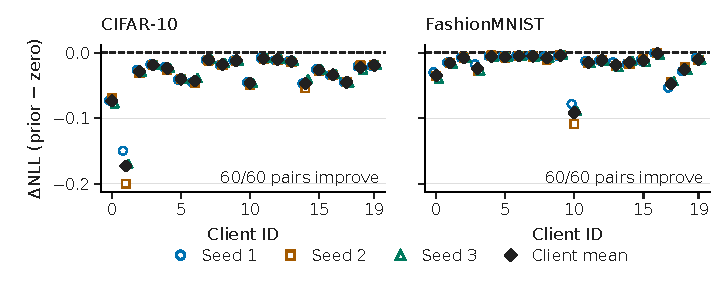
\includegraphics[width=\linewidth]{figures/clients_route_a.pdf}
\caption{Prior centering lowers NLL in every original pair. Three seed markers per client show prior-minus-zero NLL; diamonds are client means.}\label{fig:clients}
\end{figure}

Learned correction reduces NLL over fixed prior addition by 0.0282/0.0222. Eleven-value same-prior BCTS comes within 0.0016/0.0036 of the vector predictor, supporting the prior center across score families.

\begin{table}[!htb]\centering\small\setlength{\tabcolsep}{2.2pt}
\caption{Prior-centered vector scaling lowers NLL and Brier score; BCTS gives lower client ECE. Upper: Brier/ECE (lower is better), ECE in percentage points. P denotes prior centering. Lower: means; accuracy is a proportion.}\label{tab:quality}
\begin{tabular}{@{}lrrr@{\hspace{3.7pt}}rrr@{}}\toprule
& \multicolumn{3}{c}{CIFAR-10} & \multicolumn{3}{c}{FashionMNIST}\\
Predictor & Brier & ECE$_c$ & ECE$_p$ & Brier & ECE$_c$ & ECE$_p$\\\midrule
Zero & $0.343\pm0.008$ & $6.15\pm0.20$ & $1.35\pm0.41$ & $0.108\pm0.006$ & $3.69\pm0.45$ & $0.58\pm0.20$\\
P-BCTS & $0.341\pm0.007$ & $5.37\pm0.23$ & $1.30\pm0.10$ & $0.105\pm0.005$ & $2.82\pm0.07$ & $0.45\pm0.21$\\
P-vector & $0.340\pm0.008$ & $5.48\pm0.17$ & $1.49\pm0.24$ & $0.103\pm0.006$ & $3.05\pm0.18$ & $0.47\pm0.20$\\\bottomrule
\end{tabular}
\par\medskip
\begin{tabular}{lrrrr}\toprule
& \multicolumn{2}{c}{CIFAR-10} & \multicolumn{2}{c}{FashionMNIST}\\
Endpoint & Zero & Prior & Zero & Prior\\\midrule
Weighted NLL & 0.6788 & 0.6571 & 0.1588 & 0.1486\\
Weighted accuracy & 0.7475 & 0.7471 & 0.9462 & 0.9473\\
Client accuracy $q_{10}$ & 0.6027 & 0.6065 & 0.8578 & 0.8566\\\bottomrule
\end{tabular}
\end{table}

The prior vector lowers mean NLL, whereas same-prior BCTS lowers mean client ECE (Table~\ref{tab:quality}). Weighted NLL falls by 0.0217/0.0102, less than the macro reductions. Sample-weighted accuracy equals pooled accuracy and changes by $-0.04$/$+0.11$ percentage points.

\subsection{Class alignment explains the informative center}

The aligned center lowers holdout NLL by 0.071145/0.043893 relative to its fixed class permutation (Table~\ref{tab:mechanism}); all sixty pairs per task favor alignment at fixed norm and capacity.

Mean probability mass on TRAIN-absent classes is 0.00279/0.03076/0.04639 for correct/zero/permuted centers on CIFAR and 0.00087/0.00912/0.01670 on Fashion. Such labels constitute about 0.019\%/0.037\% of holdouts, making suppression a trade-off.

\paragraph{Penalty sensitivity.}
Development NLL is close across $\lambda\in\{0.1,1,10\}$ and rises toward fixed prior addition (Fig.~\ref{fig:lambda}); we retain $\lambda=10$. Appendix~\ref{app:sensitivity}, Diagnostics, reports frozen-center reallocation. All nine development configurations across three label-skew partitions per task favor prior centering; the CIFAR-100 extension lowers NLL from 2.4283 to 2.2896 with 800 B of local state (Table~\ref{tab:partitiondev}).

\begin{figure}[!htb]\centering
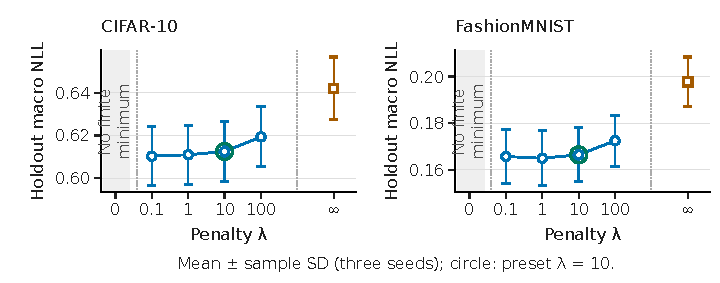
\includegraphics[width=\linewidth]{figures/lambda_route_a.pdf}
\caption{Finite correction lowers development NLL below fixed-prior addition. Markers/bars: three-seed mean/sample SD; original $\lambda=10$ retained. Missing classes prevent a finite $\lambda=0$ minimum.}\label{fig:lambda}
\end{figure}

\subsection{Predictive quality under compressed shared training}

Ordinary CE and the count-adjusted training loss produce close results with the same predictor (Table~\ref{tab:training}); the training loss is not the method contribution.


Table~\ref{tab:reference} reports the same-budget compressor and persistent-personalization references; prior centering also reduces NLL relative to zero-centered fits on dense FedAvg and FedProx (Table~\ref{tab:dense_baselines}). The matched pFedMe adapter gives NLL 1.0072/0.3557 at five inner gradients per batch and dense communication (Appendix~\ref{app:complete}).

Uniform3 uploads 54,067 B (scales/header included), 90.13\% below the analytical 547,560 B dense profile. Retaining dense downlinks reduces upload--download traffic from 1,095,120 B to 601,627 B (45.06\%). Predictor state costs 80 B (BCTS: 44 B; Linear/residual head: 2,600 B); each client retains a 547,496 B residual.


